\documentclass[12pt]{article}

% USEPACKAGES
\usepackage[margin=2.5cm]{geometry} % Change border margins.
\usepackage[titles]{tocloft} % Table of Contents, manual add.
\usepackage{mcode} % Load matlab code into LaTeX.
\usepackage[parfill]{parskip} % Removes indents
\usepackage[hidelinks]{hyperref} % Clickable links in PDF.
\usepackage{fancyhdr}
\usepackage{graphicx}
\usepackage{epstopdf}
\usepackage{float}
\usepackage{amsmath,amssymb,amsthm,multirow,algorithm,algorithmic,amsfonts}
\usepackage{gensymb}
\usepackage[square,numbers,comma,sort&compress]{natbib}
\usepackage[titletoc]{appendix}
\usepackage[final]{pdfpages}
\usepackage{afterpage}
\usepackage{mdwlist} % Compact lists (itemize*)
\usepackage{fixltx2e}
\usepackage[table]{xcolor}
\usepackage{expl3}
\usepackage[nogroupskip,acronyms,symbols]{glossaries}
\usepackage{glossary-longragged}
\usepackage{wrapfig}


\usepackage{lscape}
\usepackage{rotating}

% PAGESTYLE
\pagestyle{plain}

% Generate the glossary
	% create a new glossary style for the list of symbols
	% copied (but eddited) from http://www.latex-community.org/forum/viewtopic.php?f=5&t=20797
	\newglossarystyle{listos}{%
	  \glossarystyle{altlongragged4col}
	  \setlength{\glsdescwidth}{0.8\textwidth}
	  \setlength{\glspagelistwidth}{0.1\textwidth}
	  % allow line wrap in the description column
	  \renewenvironment{theglossary}%
	    {\begin{longtable}{llp{\glsdescwidth}p{\glspagelistwidth}}}%
	    {\end{longtable}}%
	  \renewcommand{\glsgroupskip}{}% make nothing happen between groups
	  % swap second and third columns
	  \renewcommand*{\glossaryentryfield}[5]{%
	    \glsentryitem{##1}\glstarget{##1}{##2} & ##4 & ##3 & ##5\\}
	  % sub-entries
	  \renewcommand*{\glossarysubentryfield}[6]{%
	     \glssubentryitem{##2}%
	     \glstarget{##2}{##3} & ##5 & ##4 & ##6\\}%
	}
\newglossary*{symbol}{List of symbols}
\makenoidxglossaries
\setacronymstyle{long-short}
\loadglsentries{./Acronyms}
\newglossaryentry{romanletter}{type=symbol,name={},description={\nopostdesc},sort=a}
\newglossaryentry{greekletter}{type=symbol,name={},description={\nopostdesc},sort=b}
\loadglsentries{./Symbols}



% COMMANDS
\newcommand{\HRule}{\rule{\linewidth}{0.04cm}}
\renewcommand{\abstractname}{{\Large Summary}}
\renewcommand{\cftsecleader}{\cftdotfill{\cftdotsep}}
\setlength{\parskip}{5pt plus4pt minus2pt}
\setcounter{tocdepth}{2}
% ENVIRONMENTS
\newenvironment{drawing}


\begin{document}
% Titlepage
\begin{titlepage}
\begin{center}

% Upper part of the page
\textsc{\LARGE Delft University of Technology}\\[0.3cm]
\textsc{\Large AE2100 Design and Construction}\\[0.5cm]

% Title
\HRule \\[0.4cm]
{\Huge \bfseries Title}\\[0.2cm]
{\Large \bfseries Subtitle}\\[0.2cm]
\HRule \\[0.9cm]

% Image
\includegraphics[scale=0.35]{./Titlepage/coverpicture}\\[0.5cm]

% Author
D.D. Hage - 4190696\\[0.3cm] A11\\[0.35cm]
\vfill

% Date
\begin{large}\today \end{large}

\end{center}
\end{titlepage}
\pagenumbering{roman}

% Summary
\newpage
\section*{Preface}\label{cha:preface}

\begin{flushright}
Delft, 23 April 2015
\end{flushright}

Dear Reader,	
\\ [1cm]
This Project Plan (PP) describes the process and results of the planning phase of the project to design an inflatable guidable aeroshell suitable for manned space flight. This project follows in the wake of a number of investigations performed by the National Aeronautics and Space Administration (NASA) in the viability of such a vehicle for entry and re-entry of atmospheres. Key driver for a new solution to (re-)entry using heat shield is a reduction of mass as compared to conventional solutions, greatly benefiting launch costs for missions to explore and inhabit extraterrestrial environments, such as Mars. 
\\ [1.5cm]
Design Synthesis Exercise Group 02
\section*{Summary}\label{cha:summary}

% Table of contents
\newpage
\tableofcontents
\addtocontents{toc}{\protect\contentsline {section}{Acronyms}{v}{}}
\addtocontents{toc}{\protect\contentsline {section}{List of symbols}{vi}{}}
\addtocontents{toc}{\protect\contentsline {section}{List of Figures}{vii}{}}
\addtocontents{toc}{\protect\contentsline {section}{List of Tables}{viii}{}}

\newpage
\printnoidxglossary[type=\acronymtype,nonumberlist]
\newpage
\printnoidxglossary[type=symbol,nonumberlist,style=listos]
\newpage
\listoffigures
\newpage
\listoftables

% Chapters
\newpage
\pagenumbering{arabic}

\section{Introduction}
\label{cha:introduction}

A controllable inflatable aeroshell has high potential to deliver sufficient aerodynamic deceleration to bring human payload to the surface of extraterrestrial locations, such as Mars, at a significantly lower mass fraction: the conventional solution, a rigid aeroshell, may have a hypersonic decelerator mass fraction of up to $30\%$. Payload-carrying capability can therefore be increased such that the economic feasibility of extraterrestrial exploration and habitation missions is significantly increased. Human interest in space exploration persists and a large number of planned human space flight missions make such a lightweight solution high in demand. 

To this end the study focuses on designing a \acrfull{cia} that brings a vehicle of $10000$ $[kg]$ to the surface of Mars, one of the most challenging environments for aerocapture due to its thin atmosphere, with a decelerator mass less than ten percent of the total vehicle mass. Comparing this to the conventional mass fraction, it is clear this is a game-changer.

This Final Report details the result of the preliminary design phase, following upon the concept selection. The best concept was selected from the five researched concepts presented in the Mid-Term Report and was designed and analysed further during the preliminary design phase. In combination with the decelerator system, mission planning has been performed to give a broad overview of the environment the spacecraft is to endure. This is summarised together with the mission requirements and scope, a market analysis, sustainable development strategy and cost breakdown structure in Chapter \ref{cha:missiondescr}.

During concept selection the stacked toroid was chosen based on its performance in the trade-off criteria, including a significantly higher \gls{trl} than the other concepts and a far lower mass than the conventional rigid concept. More details on the concept selection and trade-off can be found in Chapter \ref{cha:conceptselection}. The definition of the system in terms of functions, requirements and subsystems can be found in Chapter \ref{cha:sysdef}. To fully understand the complete system and what requirements are imposed on the decelerator, the crew module is sized as well. The crew module design is detailed in Chapter \ref{ch:crewmod}.

%The further analysis performed on the stacked toroid allows for a mass and performance estimation. 
The orbit is specified such that the maximum deceleration time can be kept, while allowing time in a parking orbit if required by unfavourable atmospheric conditions on Mars. The \gls{tps} is sized using the 1D heat equation, and using state-of-the-art materials resulted in an extremely light lay-up. The inflation structure is sized using a parametric mass model in combination with a truss-based model to estimate internal loads. Aerodynamic performance was estimated using modified Newtonian flow theory, and the shape was optimised to perform according to requirements. These tools, along with design parameter sensitivity, are presented in Chapter \ref{cha:designpar}.

The tools and sensitivity analyses are required to iterate efficiently towards a design that fulfils the requirements. A final design was formulated that complies with requirements. The iterative approach to design and the final result is detailed in Chapter \ref{cha:finaldesign}.

Finally, recommendations for future work are made, looking at the planning of activities that have to be performed from preliminary design until the end of mission. Also areas of low \gls{trl} that require further research are discussed and a strategy for verification and validation is presented.


%Concepts follow from a structured \acrfull{dot} and are characterised by their shape. This step of concept generation has yielded one rigid concept and four inflatable concepts, namely the stacked toroid, tension cone, trailing ballute and isotensoid. Concepts are evaluated for the following trade-off criteria: decelerator mass, development risk, deceleration time and stability. To the end of providing estimations that allow comparison for the five concepts in these aspects the following tools have been developed: a parametric structural mass model, a basic thermal analysis tool, an astrodynamic tool with implemented control system and an aerodynamic tool. The mass of the concepts is distinguished by three mass components, namely control system, structures and \acrfull{tps}. On the basis of the structural, astrodynamic and thermal models masses for the three mass components are estimated and compared. Development risk of concepts is estimated on the basis of past and current research into the concepts and reflected by the \acrfullpl{trl}. Deceleration time and stability are reflected by the lift-to-drag ratio and static stability coefficients respectively which are output of the aerodynamic analysis tool. On the basis of this evaluation, a trade-off is made in the \gls{mtr} in cooperation with the customer.

%An overview of the time-sequenced mission operations is given in Chapter \ref{cha:opseg}. Chapter \ref{ch:wdd} gives a definition of past, current and future work and discusses resource allocation along with the appointment of managerial and technical functions. Chapter \ref{ch:sustain} presents an approach with respect to sustainable development.  Concept trade-off criteria are presented in Chapter \ref{ch:tradeoff} and the concepts are evaluated in terms of these criteria in Chapter \ref{ch:options}. For an efficient design and the identification of iteration loops, Chapter \ref{ch:di} defines subsystem interactions. Chapters \ref{ch:astrocontrol} up to and including Chapter \ref{ch:thermtool} discuss tool development and concept evaluation in terms of trajectory, aerodynamic performance and structural and thermal mass. A risk assessment is performed in Chapter \ref{ch:riskestimation}. A summary of findings on concept performance in the trade-off criteria is given in Chapter \ref{ch:tfsum}. The report is concluded by Chapter \ref{cha:conclusion}.

%Before human interplanetary spaceflight can be achieved technological gains have to be made in several fields. One of these fields comprises hypersonic deceleration systems. Significant weight gains are expected to be possible by using inflatable aeroshells.

%However, the development of a controllable inflatable aeroshell is very complex and involves many different disciplines. 

%To reduce the complexity of designing such a system first a \acrfull{pp} was made. Following that a \acrfull{br} was produced, in order to survey the current technology state and knowledge on this subject. Now a \acrfull{mtr} report is made in order to perform a concept trade-off. 



%The purpose of this report is to present several concepts for a controllable inflatable aeroshell and to determine which concept is best suited for performing the design mission. First the group organisation for the period between the \acrlong{mtr} and \acrlong{fr} is discussed in chapter \ref{ch:wdd}, including individual and group tasks and work packages. A \acrfull{wbs} is made, together with a \acrfull{wfd} and Gantt chart. Secondly the approach with respect to sustainable development is presented in chapter \ref{ch:sustain}. Thirdly the \glspl{dot} are used in chapter \ref{ch:options} to generate several system concepts. These concepts will be analysed with tools from several different disciplines. These consist of an astrodynamics \& control tool, as well as tools for concept mass estimation, aerodynamical characteristics and thermodynamic behaviour. The development, verification, validation of these tools is discussed in chapters \ref{ch:astrocontrol}, \ref{ch:strucmass}, \ref{ch:aero_analysis} and \ref{ch:thermtool} respectively. These chapters also show the results obtained from analysing the proposed system concepts. After the tool development and concept analysis the risk inherent to each system concept is considered in chapter \ref{ch:riskestimation}. This will be done by making a risk map for each concept. Finally the concept trade-off will be performed in chapter \ref{ch:tradeoff}, based on results of the analyses conducted in the previous chapters. The result of this is a complete trade-off matrix, after which the customer will be able to select the preferred concept based on the weights they attach to each trade-off criterion.
\section{Literature Review}\label{cha:litreview}
This chapter provides an overview of findings of literature research on the topic of (re-)entry vehicles. Firstly, past solutions and their development have been investigated for the dual purpose of reference material to be used for preliminary sizing and design and the acquisition of knowledge on mission level. Secondly, each of the primary disciplines involved in the design of a re-entry mission is investigated, namely structural design, \gls{tps}, aerodynamical design, orbital mechanics, atmospheric modelling and control. These disciplines are investigated in terms of their application and new technologies (e.g. the materials typically used for thermal protection) as well as for methods used in their respective analysis and design (e.g. the use of \gls{fem} for structural analysis).

This chapter is structured as follows. The first section gives an overview of past re-entry vehicles; the second section gives an overview of past and ongoing investigations in the use of inflatable aeroshells; subsequent sections focus on the primary distinguishable disciplines involved.

\subsection{Overview of present and past (re-)entry vehicles}\label{cha:past missions}
<<<<<<< HEAD
This section gives an overview of (re-)entry vehicles, primarily to obtain a set of reference vehicles to aid design and sizing of the payload capsule in later stages and additionally to review solutions used in the past to perform (re-)entry for human spaceflight. At this point no structure supporting the deceleration has been chosen yet, as such only payload capsule size parameters are considered. It can be argued, based on human constraints, that the attached payload capsule for this mission will have similar characteristics. Table \ref{tab:refmis} displays some characteristics related to the payload capsule which can be used as indicative values\footnote{Principal values from: \\
URL: http://www.nasa.gov/sites/default/files/167718main\_early\_years.pdf,  Accessed: 28 April 2015 \\ URL: http://www.braeunig.us/space/  Accessed: 28 April 2015 \\ URL: http://wsn.spaceflight.esa.int/docs/Factsheets/35\%20Soyuz\%20LR.pdf Accessed: 28 April 2015
}
. For the descent module a separate retropack may be installed as was the case with the Gemini and Mercury missions.
=======
This section gives an overview of (re-)entry vehicles, primarily to obtain a set of reference vehicles to aid design and sizing of the payload capsule in later stages and additionally to review solutions used in the past to perform (re-)entry for human spaceflight. At this point no structure supporting the deceleration has been chosen yet, as such only payload capsule size parameters are considered. It can be argued, based on human payload constraints, that the attached payload capsule for this mission will have similar characteristics. Table \ref{tab:refmis} displays some characteristics related to the payload capsule which can be used as indicative values. 

>>>>>>> 0c3722e462c2edef474bc86fadfa037792f5ae48

\begin{table}[H]
	\caption[Reference missions for payload module sizing]{Reference missions for payload module sizing.}
		\begin{tabular}{|p{0.18\textwidth}|p{0.11\textwidth}|p{0.11\textwidth}|p{0.11\textwidth}|p{0.11\textwidth}|p{0.11\textwidth}|p{0.11\textwidth}|} % MAKE SURE THAT THE TOTAL WIDTH IS 0.95\textwidth!! (that way its exactly the textwidth.... haha) 
			\hline
			Mission 						& Apollo & 	Soyuz TMA &	Shenzhou & Gemini & Mercury & Orion \\ \hline \hline
			Years [$yr$]					&	1964-1975	& 	2010-2014&	1999- &   1959-1963  & 1959-1963 & Future \\ \hline
			Reentry module mass [$kg$]  	&	5806& 	2900 &	3240 & 3402 & 1118 & 8777 \\ \hline
			Habitable volume [$m^3$]		&	6.17& 	3.5  &	6.0  & 2.55 & 1.9 & 11   \\ \hline
			Diameter [$m$]			 		&	3.9 & 	2.17  &	2.52 & 2.3 & 1.9 & 5   \\ \hline
			Length  [$m$]			 		&	3.5 & 	2.24  &	2.5  & 3.4 &  5.2 & Unknown  \\ \hline
			Crew size (max) [$persons$]		&	3   & 	3     &	3    & 2   &  1   & 6   \\ \hline
		\end{tabular}
    \label{tab:refmis}
\end{table}


<<<<<<< HEAD
It must be noted that table \ref{tab:refmis} displays typical values only to be used as first indicative values. For example the diameter is typically a maximum value since no single value can be supplied due to the cone like shape of most reentry vehicles. Moreover these design include the size and mass of the deceleration mission of which the latter typically includes a heavy duty heat shield. Most reentry vehicle base designs were used multiple time with minor design changes and a single externally communicated design name. As such the values in the table above should be used with proper care as indicative values only. Habitable volume estimation also depends on the mission duration and may be considerable. A study on the estimation of these parameters is given by \cite{Rudisill2008}. Al tough this study focuses on a lunar mission/base it still underlines many of the important aspects with respect to payload module sizing which are applicable for mars mission as well. It may a such prove as proper foundation for payload module sizing. 
=======
It must be noted that table \ref{tab:refmis} displays typical values only to be used as first indicative values. For example the diameter is typically a maximum value since no single value can be supplied due to the cone like shape of most reentry vehicles. Moreover these designs include the size and mass of the deceleration mission of which the latter typically includes a heavy duty heat shield. Most re-entry vehicle base designs were used multiple times with minor design changes and a single externally communicated design name. As such the values in the table above should be used with proper care as indicative values only. Habitable volume estimation also depends on the mission duration and may be considerable. A study on the estimation of these parameters is given by \cite{Rudisill}. Although this study focuses on a lunar mission it still underlines many of the important aspects with respect to payload module sizing which are applicable for Mars missions as well. It may as such prove a proper foundation for payload module sizing. 
>>>>>>> 0c3722e462c2edef474bc86fadfa037792f5ae48

From the above mentioned reference missions in table \ref{tab:refmis} especially the future Orion mission, currently being designed, is of great interest.  [GIVE AN EXPLANATION]

\subsection{Review of inflatable aeroshell technology}\label{sec:aeroshells}
This section gives an overview of the bistorical and present application of (controllable) inflatable aeroshell technology. This serves to provide an overview of the current state-of-the-art of inflatable aeroshell technology and applications, its potential advantages over traditional rigid aeroshells and a collection of literature to use for further investigation.

\subsubsection{Advantages of inflatable aeroshells}
Inflatable aeroshell systems provide the following advantages with respect to traditional rigid aeroshells \cite{Cassapakis1995, Hughes2005}:
\begin{enumerate}
\item A lower weight is typically achieved, as investigated by Cianciolo et al \cite{Cianciolo2010};
\item An (in principle) unconstrained inflatable diameter, by the launch vehicle fairing, allows use of larger aerodynamic decelerators. As a result a lower \gls{bc} is achievable;
\item A smaller aeroshell volume fraction is required as a consequence of a lack of need to use a backshell to protect the payload from aft side heating (in contrast to rigid aeroshells);
\item Effective cocooning of the payload by a rigid aeroshell diminishes accessibility. Adding access ports requires the use of additional verification and validation of thermal control design. This is not required for an inflatable aeroshell \cite{Johnson1997};
\item Heat is trapped by a rigid aeroshell cocooning the payload, causing potential interference with on-board payload thermal requirements. For an inflatable aeroshell without backshield, this is not the case.
\end{enumerate}
Of these reasons, the first two prevail for the current mission in view of constraints by the launch vehicle, limiting entry vehicle mass and diameter. A way of handling the diameter constraints, one in the launcher fairing shroud and a more relaxed one after decoupling of launcher and entry vehicle, is utilizing deployment mechanisms. These may be either mechanical or inflatable. Comparison of these two concepts yields the following characteristics in favour of inflatable structures \cite{Cassapakis1995}:
\begin{enumerate}
\item Inflatables have a high reliability of deployment due to a self-correcting system;
\item Use of thin materials obtaining strength from inflation gas pressure reduces the weight required for inflatable systems compared to mechanical structures;
\item Packaging efficiency is higher for inflatable structures than for mechanical erectable structures;
\item Loads are absorbed over a large surface area for inflatable structures, as opposed to typical load concentrations in mechanical systems. Load concentrations require local addition of weight, typically resulting in a heavier structure;
\item Inflatables typicall have a lower production cost;
\item Easily adapted to concave shapes with symmetric and curved surfaces;
\item The nearly constant inflation pressure induced force restoring encountered surface distortions is favourable for vehicle dynamics;
\item A favorable thermal response by radiation exchange over a large area.
\end{enumerate}

\subsubsection{Investigation of inflatable aeroshell technology}
The aforementioned reasons, primarily lower weight and higher packaging efficiency, have been key drivers in past and ongoing research in the use of inflatable structures for use in aerodynamic deceleration during (re-)entry. Primary contributor is the \gls{nasa}, specifically the NASA Langley Research Center, responsible for a series of tests on the feasibility and use of \gls{hiad} concepts for entry and re-entry \cite{Hughes2005, Dillman2010, Dillman2012, Dillman2014}. A brief discussion on these tests follows. Little information on gls{irve}-I \cite{Hughes2005} is present, hence it is not included in the following discussion.  

\gls{irve}-II, launched in 2009, successfully met its objectives, namely: "to demonstrate inflation and re-entry survivability, assess the thermal and drag performance of the re-entry vehicle and to collect flight data for comparison with analysis and design techniques used in vehicle development" \cite[p.1]{Dillman2010}. IRVE-II consisted of a rigid, cylindrical centerbody with a deployable, conical inflatable aeroshell of a so-called stacked toroid configuration \cite{Smith2010,Bose2009}.

IRVE-III, launched in 2012, had as primary aim to demonstrate the offset of the vehicle \gls{cg} on the lift-to-drag ratio of the vehicle and demonstrate survability with flight-relevant heating \cite{Dillman2012a}. The configuration was similar to IRVE-II and subsystems were altered predominantly in the following  manners \cite{Dillman2012a}:
\begin{itemize}
\item Support straps were added to inter- and intraconnect toroids and centerbody;
\item The \gls{tps} was upgraded by use of a multi-layer system, consisting of two layers of Nextel fabric, Pyrogel insulation and a Kapton/Kevlar thin film gas barrier, in place of the Nextel fabric used in IRVE-II \cite{Dillman2012}; 
\item A heater was added to the pressure tank system used to inflate the stracked toroid structure;
\item The addition of a \gls{cg} offset mechanism to alter the lifting behavior of the vehicle and thereby control it.
\end{itemize}
IRVE-III succeeded in its goals, demonstrating the feasibility of a \gls{cg} offset for vehicle control \cite{Dillman2012}.

\gls{thor}, planned for launch in 2016, features a more blunt aeroshell with a half-cone angle of 70 instead of 60 degrees, to analyze stability and drag differences with previous configurations \cite{Hughes2005, Dillman2010, Dillman2012, Dillman2014}. In addition, it features Zylon instead of the Kevlar fibres used for IRVE-III, allowing a thinner \gls{tps} layup of a different composition. In terms of \gls{tps}, silicon carbide fabric over carbon felt insulation is used instead of Nextel fabric over Pyrogel insulation \cite{Dillman2014}.

In addition to these flight tests, ground testing has been pursued in parallel to further technology developments for \gls{hiad} application \cite{Smith2010}.

Some of the most important characteristics of the re-entry vehicles during these missions are displayed in Table \ref{tab:hiadcomparison}.

\begin{table}[h!]
	\caption{Comparison of recent HIAD missions} \label{tab:hiadcomparison}% LABEL HERE
		\begin{tabular}{|p{0.28\textwidth}|p{0.08\textwidth}|p{0.15\textwidth}|p{0.15\textwidth}|p{0.21\textwidth}|} % MAKE SURE THAT THE TOTAL WIDTH IS 0.95\textwidth!! (that way its exactly the textwidth.... haha) 
			\hline

       Mission parameter   &       Unit &     IRVE-II \cite{Dillman2010} &     IRVE-III \citep{Dillman2012,Dillman2014} & THOR (predicted) \citep{Dillman2014} \\
			\hline \hline

Launch date &          [-] & 17-08-2009 & 23-07-2012 &       2016 \\
			\hline

      Mass &         [kg] &    124.6 &        280 &        315 \\
			\hline

Shell diameter &          [m] &       2.93 &       2.93 &        3.7 \\
			\hline

Shell angle &     [deg] &         60 &         60 &         70 \\
			\hline

    Apogee &         [km] &        218 &        469 &    200-250 \\
			\hline

Peak dynamic pressure &         [Pa] &       1180 &   Unknown         &   Unknown         \\
			\hline

Peak stagnation heating &     $ [\frac{W}{cm^{2}}]$ &        2.2 &       14.4 &         65 \\
			\hline

Peak temperature &          [C] &        100 &        378 &      Unknown      \\
			\hline

Peak Mach Number &          [-] &        6.2 &  Unknown          &   Unknown         \\
			\hline

Maximum deceleration &          [g] &        8.5 &       20.2 &       8-10 \\
			\hline

		\end{tabular}
    
\end{table}


\subsection{Structures in (re-)entry vehicles}\label{sec:struc}
Applications and technologies, within the field of structures and materials, as applied in (re-)entry vehicles are investigated, with an emphasis on inflatable aeroshells. These are investigated firstly for non-inflatable structures and secondly for inflatable structures.

\subsubsection{Non-inflatable structures}
Non-inflatable structures can be either deployable or non-deployable. Conventional solutions, such as the Apollo or Soyuz capsule, employ a non-deployable heat shield. An advantage of a deployable heat shield is effecting a larger surface area for aerodynamic deceleration. In most cases, this is supplemented by retropropulsive means.



\subsubsection{Inflatable structures}
The inflatable aeroshell system implemented in the \gls{irve} satellites mainly consists of four sub-elements: an inflatable bladder, containing a pressurised medium, a structural restraint, gas barrier and a thermal protection layer \cite{Hughes2005}. In addition, this bladder may be further subdivided into isolated volumes to provide avoid \gls{spfs}. After flow initiation with pyrotechnic valves the gas flows from the storage tank to the inflatable bladder. This flow is protected by gas valves to prevent backflow from the bladders. \cite{Hughes2005} 

In terms of the inflation process, the pressure and gas used for inflation are variable. The IRVE satellites featured nitrogen gas (and subliming powders), with an operating pressure of 3000 psi for IRVE-4 \cite{Litton2011}. An alternative to the use of nitrogen gas is hydrazine, typically capable of delivering lower weight and volume, at the expense of handling, safety and cost \cite{Freeland1998}. Estimating the required minimum pressure can be done using references \cite{Samareh2011, Brown2009}.

In addition to pure inflation, rigidization may be applied. Rigidization stiffens the structure after inflation, a process that may be performed by multiple techniques. These techniques are described in Ref. \cite{Freeland1998,Jenkins2001}, for example using fibres impregnated with a resin that cures at a certain temperature. 






Inflatable structures may be preferable to conventional non-inflatable structures for a number of structural reasons. Most importantly inflatable structures typically have a lower weight. A weight estimation method for multiple types of inflatable deceleration mechanisms is provided by \cite{Samareh2011}.







\subsection{Aerodynamics for (re-)entry vehicles} \label{sec:aero}
Hypersonic aerodynamics is a complex field of study. Ground testing is difficult, as the high temperatures experienced during hypersonic flight may damage testing facilities \cite{AndersonJr.2006, Bertin1994}. For the solution of the full flow field around a body in hypersonic flow, \gls{cfd} is required. This solution requires significant knowledge of the problem to implement, is computationally expensive and difficult to validate \cite{AndersonJr.2006, Bertin1994}. A useful engineering method for determining the aerodynamic characteristics of an arbitrary body in hypersonic flow is the (modified) Newtonian theory. It provides an acceptable approximation of the pressure distribution on the side of the body exposed to the free stream. From this pressure distribution aerodynamic coefficients can be determined. As long as the body drag is dominated by the pressure drag, the modified Newtonian method provides a good approximation of the body drag coefficient \cite{AndersonJr.2006, Bertin1994, Bertin2006}. Bodies with a high ballistic coefficient experience higher peak heat loads. This has led to the development of blunt (re-)entry vehicles \cite{Bertin1994,Theisinger2009}. A method for determining an optimal shape for a (re-)entry vehicle is presented in Ref.\cite{Theisinger2009}. A non zero $\frac{\gls{sym:L}}{\gls{sym:D}}$ ratio allows downrange and cross range control of a reentry vehicle \cite{Theisinger2009}. Hypersonic flows show an interesting characteristic known as Mach number independence; the aerodynamic coefficients of a body in hypersonic flow (\gls{sym:M}$>$5) are independent of Mach number \cite{Bertin1994,AndersonJr.2007,Hollis}. No analytical engineering method exists for supersonic flow around a blunt body. An implementation of a time marching finite difference scheme is proposed in references \cite{AndersonJr.2007} and \cite{AndersonJr.2006} to describe the flow field around an arbitrary body in supersonic flow. 

The aerothermodynamics of hypersonic flight are complex. In contrast with subsonic and supersonic aerothermodynamics during hypersonic flight also internal chemical reactions and gas composition changes occur  because of the high temperatures encountered \cite{AndersonJr.2006}. This significantly increases the computational cost of \gls{cfd} methods. In order to estimate the heat flux into the vehicle body therefore the approximate method outlined in \cite{Tauber1986,AndersonJr.2006} is proposed. This method uses the same input parameters as the modified Newtonian method that will be used for the drag estimation and is adaptable to both laminar and turbulent flow around arbitrary bodies in hypersonic and supersonic flows. From this method it follows that the local heat flux into the arbitrary body is dependent on the freestream density \& velocity as well as on local body angle with respect to the undisturbed freestream flow, distance measured along the body surface from the stagnation point and local entropy ratio between the wall and total conditions \cite{Tauber1986, AndersonJr.2006}.
\section{Trajectory analysis} \label{ch:trajectory}

**intro**

\subsection{Governing equations}\label{sec:gov}

\begin{wrapfigure}{r}{0.4\textwidth}
		\centering
		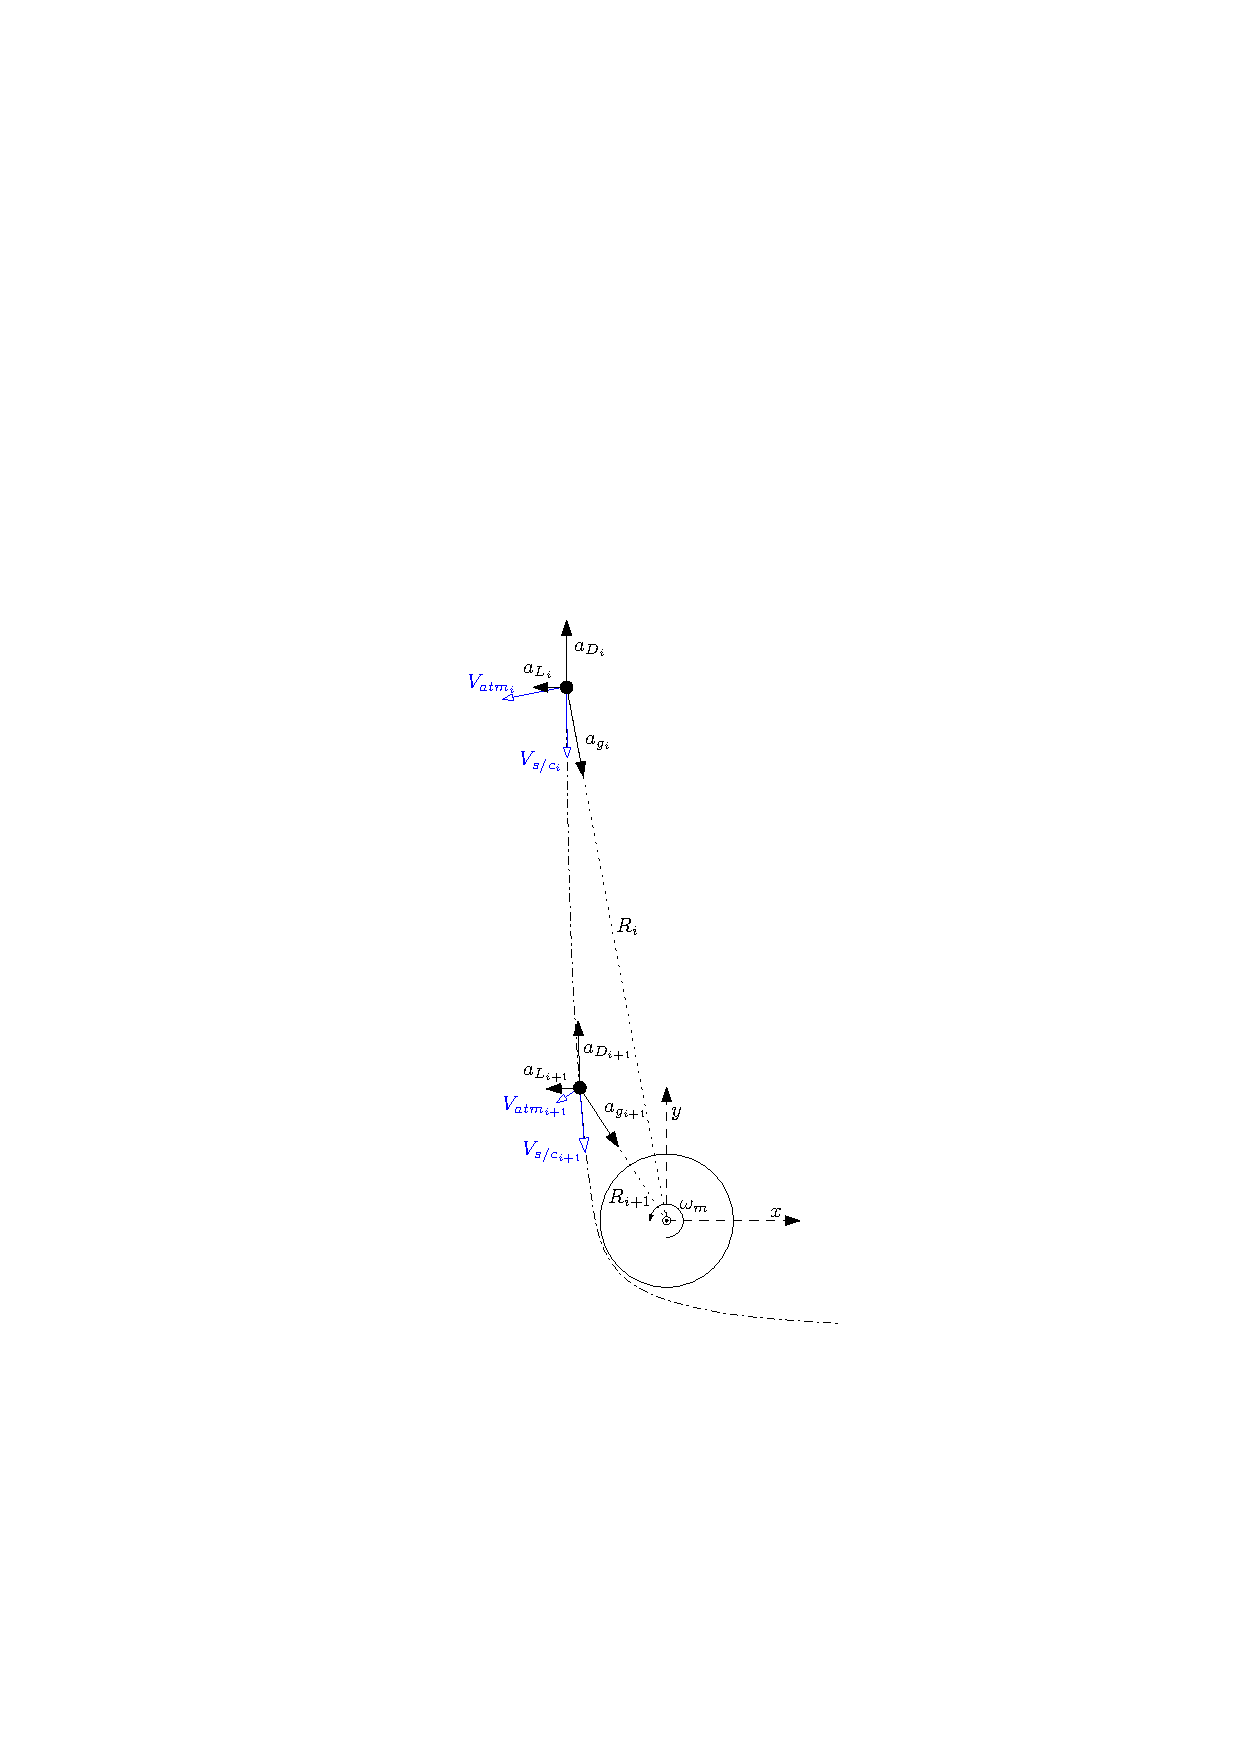
\includegraphics[width = 0.4\textwidth]{Figure/orbital_mechanics.pdf}
		\caption{The \gls{fbs} of the aeroshell mission}
		\label{fig:orb}
\end{wrapfigure}

The motion of a spacecraft can be broken down in some dominant contributors. These contributors are the gravitational pull and the aerodynamic forces. Disturbances like solar radiation or gravitational pull from moons or other bodies is neglected in the model.

The gravitational pull is described by Newtons law of gravitation

\begin{equation}
\gls{sym:F} = \gls{con:G}
\end{equation}

\subsection{Program structure}\label{sec:prog_struct}

In order to use the governing equations (equation \ref{eq:final}**!!need label!!**) to produce usefull results they have to be implemented in a simulation which calculates the trajectory. From this calculated trajectory the program has to extract usefull data and conclusions. To model aerodynamic forces on the spacecraft an atmosphere model is needed. The atmosphere model used is presented in subsection \label{subsec:atmos}. The three different modules comprising the program are discribed in subsection \ref{subsec:modules}. In subsection \ref{subsec:flow} a flowchart of the program is presented.

\subsubsection{Atmosphere model}\ref{subsec:atmos}
**inputs
**basic working principle
**outputs
**implementation in program
\subsubsection{Modules} \label{subsec:modules}

The program first implements the governing equations on each time step. Secondly two modules were created, one to find feasible orbits and another to calculate the full orbit of the orbits which are found to be feasible. These three modules are described below.

\paragraph{Implementation of governing equations}\textit{orbit.m}

The module implementing the governing equations has a lot of input data of which most are constants and vehicle parameters. One of the inputs is the dataset created by the atmospheric model described in subsection \ref{subsec:atmos}. The density and gravitational acceleration taken from this dataset is different for each cycle of the program and dependent on the height, longitude and latitude of the spacecraft. Also the previous location, velocity and acceleration (in vector form) are constantly changing inputs.

The input variables are directly filled in into equation \ref{eq:final}. This creates output values for the location, velocity and acceleration. Both the total acceleration and the separate accelerations due to the drag, lift and gravitation are outputted.
\paragraph{Orbit selection} \textit{orbit\_selection.m}

**input

In the module for orbit selection first the initial conditions are created. One of the initial conditions is that the entry velocity is $7 \frac{km}{s}$. After this initialization \textit{orbit.m} is called for each time step. After each time step the data is analyzed and three conditions are filled in. The condition \textit{inatmos} is true when the spacecraft has ever been inside the atmosphere of mars. The condition \textit{crash} is true when the spacecraft touches the surface of mars in the first entry into the atmosphere. Finally the condition \textit{inorbit} is true when the spacecraft either leaves the atmosphere with a velocity smaller than the escape velocity at that point or when the spacecraft did never enter the atmosphere and the velocity at the point the simulation is terminated is smaller than the escape velocity at that point. The values of these conditions is used in \textit{orbitcheck.m} to determine the feasible initial conditions.

**output

\paragraph{Full orbit simulation} \textit{orbit\_full.m}

**

\paragraph{Run orbit selection} \textit{orbitcheck.m}

**

\subsubsection{Flowchart} \label{subsec:flow}
**flowchart

\begin{figure}[H]
\centering
\hspace{-23mm}
\includegraphics[width = 0.8\textwidth]{Figure/astro_tool.pdf}
\vspace{-5mm}
\caption{Flowchart of the working principle of the trajectory analysis program}
\label{fig:traj_flow}
\end{figure}

\subsection{Verification and validation}
\section{Functional analysis}\label{ch:func}

\begin{figure}[H]
\centering
\includegraphics[width = 1.2\textwidth]{Figure/FFD.pdf}
\caption{Functional Flow Diagram (FFD) of aeroshell mission.}
\label{fig:ffd}
\end{figure}
\section{Requirement analysis} \label{ch:req}
This section will analyze the requirements of the re-entry mission. It will start by providing a requirement breakdown structure, which visualizes the way the different requirements on the re-entry vehicle flow down from the top level mission requirements and constraints. This will be followed by an analysis of the subsystem requirements. This analysis will follow from the flown down presented in the requirements breakdown structure. Finally, the requirements will be precisely defined and documented. The output of this final step will be the requirements used during the product design. %Guido: Dit moet nog beter geformuleerd worden, maar kon even niets beters bedenken

\subsection{Requirement Breakdown Structure}
The overarching mission requires the system to perform a manned re-entry on Mars. Several performance requirements and mission constraints are imposed on the system. These overall requirements and constraints were detailed in the project plan \cite{Balasooriyan2015}. From these overall requirements and constraints, subsystem requirements can be derived. Figure \ref{fig:RBS} graphically displays this requirement breakdown, and provides a sample parameter which has a requirement imposed on it due to the top level requirements. Each of the subsystems' requirements will be elaborated and expanded upon in the remainder op this section. 

\begin{figure}[h]
\centering
\includegraphics[width=0.95\textwidth]{Figure/RBS.pdf}
\caption{Requirements Breakdown Structure} \label{fig:RBS}
\end{figure}

\subsection{Aerodynamic Requirements Discovery} 
\label{sec:aero}
%A number of aerodynamical requirements can be seen in figure \ref{fig:RBS}. These will all be discussed here, together with their origins and impacts.

%\textbf{Decelerate within 10 days}\\
%From the limited amount of time available for the deceleration a minimum 

%\textbf{Decelerate without excessive heating}\\
%In order to guarantee the safety of the astronauts onboard the spacecraft the spacecraft cannot be heated excessively. Since this heat is caused by the drag exerted on the spacecraft this imposes a constraint on the maximum allowable heat flux produced by said drag. 

%\textbf{Decelerate in a controlled manner}\\
%To make sure that the spacecraft is controllable during the deceleration procedure 

\begin{table}[h]
	\centering
	\caption{Overview of functional requirements on aerodynamical characteristics}
	\label{tab:aeroreqs}
	\begin{tabular}{|c|c|}
		\hline
		\textbf{ID} & \textbf{Description} \\
		CIA-B07-Aero-01 & The system shall produce no more drag than that which causes a deceleration of 3 Earth g's\\
		CIA-B08-Aero-01 & The system shall produce drag sufficient to complete the deceleration within 10 Earth days \\
		\hline
	\end{tabular}
\end{table}
\subsection{Structural Requirements Discovery} \label{sec:struct}
The vehicle structure faces a number of requirements, functional and operational. The following functional requirements apply to the structures subsystem

\begin{table}[H]
	\caption{Overview of functional requirements on structures subsystem}
	\begin{tabular}{|p{0.20\textwidth}|p{0.70\textwidth}|}
    \hline
    ID          & Description                                                                                                      \\ \hline \hline
    CIA-B01-Struc-01 & The structure shall operate at least within a temperature range of [\gls{tbd},\gls{tbd}] degrees Celsius           \\ \hline
    CIA-B02-Struc-02 & The structure shall support deployment functionality \\ \hline
    CIA-B07-Struc-03 & The structure shall withstand loads of at least 3g in each axis without failure                           \\ \hline
    CIA-B09-Struc-04 & The structure shall connect payload and deceleration mechanism \\ \hline
    \end{tabular}
    \label{tab:strucfuncrequirements}
\end{table}

\begin{table}[H]
	\caption{Overview of operational requirements on structures subsystem}
	\begin{tabular}{|p{0.20\textwidth}|p{0.70\textwidth}|}
    \hline
    ID          & Description                                                                                                      \\ \hline \hline
    CIA-B02-Struc-05 & The structure shall have a maximum diameter not exceeding 12 [m] in deployed configuration     \\ \hline
    CIA-B03-Struc-06 &  The structure shall have a maximum diameter not exceeding 5 [m] in stowed configuration                              \\ \hline
    CIA-B04-Struc-07 & The structure shall have a mass not exceeding \gls{tbd} [kg]\\ \hline
    \end{tabular}
    \label{tab:strucoprequirements}
\end{table}
\subsection{Thermal Protection Requirements Discovery} \label{sec:therm}
The requirements for the thermal subsystem flow down from the \gls{rdt} and are listed in Table \ref{tab:thermalreq}. The requirements are split up in two parts, the \gls{tps} and the \gls{tcs}. The \gls{tps} mainly distributes the heat load and flux generated by decelerating the re-entry vehicle, whereas the \gls{tcs} controls the temperature of the payload and other subsystems.


\begin{table}[H]
	\caption{Overview of thermal requirements}
	\begin{tabular}{|p{0.25\textwidth}|p{0.70\textwidth}|}
    \hline
    ID          & Description                                                                                                      \\ \hline \hline
    CIA-B01-TPS-01 & The TPS shall be able to withstand the maximum heat flux of \gls{tbd} $ \left[\frac{W}{cm^2}\right] $.               
\\ \hline
    CIA-B01-TPS-02 &  The TPS shall be able to withstand the maximum heat load of \gls{tbd} $ \left[\frac{J}{cm^2}\right] $.                
\\ \hline
    CIA-B01-TCS-01 & The TCS shall keep the payload and other subsystems within a specified temperature range in $\left[^{\circ}C\right]$.                                            
\\ \hline
    \end{tabular}
    \label{tab:thermalreq}
\end{table}

The first requirements 

The second requirement

The payload and subsystems are only able to withstand a certain temperature range. To keep the payload and subsystems within this range the TCS follows requirement CIA-B01-TCS-01.
In this section the methods used for determining appropriate control systems are explained. These systems should be able to keep the spacecraft on the trajectory as defined by the astrodynamics tool in section \ref{subsec:orbittool}. First the assumptions used and their effects on the accuracy of the analysis are explained. Than a point is determined

\paragraph{Assumptions}

**Primary and Secondary assumptions**

\paragraph{Trim point}

**Moment equilibrium figures/equations**
**CG-location plot(s)  with conclusion on CG for AoA~20 and sideslip angle=0**

\paragraph{Stability}

**From E.Mooij**

\paragraph{Available control systems}

**Intro**

\subparagraph{\acrfull{cg} offset}

**Not nessesary for AoA, not feasible for sideslip**

\subparagraph{Thrusters}

**Sebstiaan**

\subparagraph{Aerodynamic surfaces}

**Guido**




\subsection{List of Requirements} \label{sec:list}

\begin{table}[H]
	\caption{Overview of mission top-level requirements}
	\begin{tabular}{|p{0.10\textwidth}|p{0.85\textwidth}|}
    \hline
    ID          & Description                                                                                                      \\ \hline \hline
    CIA-A01 & The re-entry vehicle shall be able to cope with an entry velocity of seven kilometers per second.                \\ \hline
    CIA-A02 & The inflated aeroshell shall have a maximum diameter of 12 meters.                                               \\ \hline
    CIA-A03 & The system shall have a diameter not exceeding 5 meters in stowed condition                                       \\ \hline
    CIA-A04 & The maximum entry mass of the re-entry vehicle shall be 10,000 kilograms at the start of the mission.				\\ \hline
    CIA-A05 & The hypersonic deceleration system mass shall not be heavier than ten percent of the total re-entry vehicle mass. \\ \hline
    CIA-A06 & The control system shall have a maximum failure probability of 5.0e-4.                                           \\ \hline
    CIA-A07 & The maximum allowable loads on the re-entry vehicle shall be 3 Earth g's in each axis.                            \\ \hline
    CIA-A08 & The re-entry vehicle shall have a maximal aerobraking duration of ten Earth days.                                      \\ \hline
    CIA-A09 & The re-entry vehicle shall support $<$\gls{tbd}$>$ humans as payload.                         				            \\ \hline
    \end{tabular}
    \label{tab:toplevelreq}
\end{table}





\section{Budget breakdown} \label{ch:budget}
\section{Market analysis} \label{ch:market}
\section{Risk assessment} 
\label{ch:risk}
This section will cover the initial risk assessment that was carried out during the conceptual design phase. First a risk map was constructed, followed by an explanation of the contingency margins that will be used during the various design phases. These are based on the outcomes of the risk assessment. Section \ref{sec:riskmap} will cover the risk map, after which section \ref{sec:tca} will discuss the technical contingency allocation.

\subsection{Risk map}
\label{sec:riskmap}
 A risk map has been constructed in order to identify which mission and design elements pose the biggest risk. From the risk map it can be seen which elements require the most attention in order to mitigate the risks they pose. The risk map is shown in table \ref{tab:riskmap}. The colors correspond to the amount of risk each table cell represents. The numbers in table \ref{tab:riskmap} correspond to the elements shown in table \ref{tab:riskelements}.

\begin{table}[h]
\centering
\caption{Risk map}
\label{tab:riskmap}
    \begin{tabular}{|c|c|c|c|c|}
    \hline
    \textbf{Feasible in theory} & & & & \\
    \textbf{Working laboratory model} & & & & \\
    \textbf{Used in-flight on Earth} & & & & \\
    \textbf{Derived from used technology on Mars} & & & & \\
    \textbf{Feasible in theory} & & & & \\
     & \textbf{Negligible} & \textbf{Marginal} & \textbf{Critical} & \textbf{Catastrophic} \\ \hline
%     \bf{Static earth} & \cellcolor{green!25}35g - 5 & \cellcolor{blue!25}0.3W - 3 & \cellcolor{red!25}1$^\circ$ - 1 & \cellcolor{red!25}39\\ \hline
    \end{tabular}
\end{table}

\begin{table}[h]
\centering
\caption{Risk map elements}
\label{tab:riskelements}
\begin{tabular}{|c|c|}
\hline
\textbf{Number} & \textbf{Element} \\
\hline
1 & Control system \\
2 & \\
3 & \\
4 & \\
5 & \\
6 & \\
7 & \\
8 & Long space exposure \\
\hline
\end{tabular}
\end{table}

\subsection{Technical contingency allocation}
\label{sec:tca}
From the risk map of the preceding section one can see that there are many
\section{Approach with respect to sustainable development}\label{cha:sustain}
Sustainable development in engineering means that the design, production, operation and disposal of a product should be done in a sustainable way. In this case sustainable means that energy and resources are used in a manner that does not threaten the environment or the needs of future generations. In this chapter the general approach with respect to the sustainable development of the controllable inflatable aeroshell is briefly discussed.

Even though sustainability is becoming more important in engineering, it is of less importance in these kind of space missions. The reason for this is that the proposed mission is a single mission and therefore its total impact will be relatively small. For example, it is acceptable that the production of the space vehicle is less sustainable than the production of one small passenger aircraft, since the aircraft is produced in large numbers whereas only one space vehicle is produced. It can therefore be said that sustainability will not be the design driver for the controllable inflatable aeroshell. Of course, sustainable methods are preferred when they do not add much costs and very unsustainable methods are to be avoided.

Some examples of sustainable methods can be mentioned. In the process of producing the aeroshell unnecessary polluting methods that threaten the natural environment should be avoided. Also interplanetary forward contamination should be prevented. In this case it means that life and other forms of contamination should not be transferred from Earth to Mars. In practice this is already standard procedure. Another, less important, form of sustainability is the avoidance of space debris in the atmospheres of Earth and Mars.

Therefore sustainability will not be a leading driver for the design of the controllable inflatable aeroshell, as long as very unsustainable methods are avoided. The latter is effected by a preference of sustainable methods in choices for production and operation of the aeroshell.
\section{Design Option Structuring} \label{ch:design}
This chapter gives an overview of initial design concept selection, focusing on the different missions aspects of XXX. This concept generation is done systematically by means of a \gls{dot} for each of the aspects. Combination of the different trees then yields a number of final concepts. The next phase is eliminating clearly unfeasible or undevelopable concepts. The chapter commences with a \gls{dot} for each of the mission aspects in subsequent sections, including eliminating unfeasible concepts.

\subsection{Deceleration mechanism}
On the basis of the ...

\subsection{Trajectory control}

\subsection{Aerodynamic deceleration shape}

%\subsection{Inflation system}
%As mentioned in Chapter \ref{cha:litreview}, inflation can be performed either with (ram-air) or without use of the atmosphere. A third option is the use of both (hybrid), thereby featuring ram-air inlets as well as internal gas storage and feed systems. In terms of the medium used for inflation, conventionally nitrogen gas is used. An alternative would be hydrazine gas, as explained in Chapter \ref{cha:litreview}.



\section{Conclusion}

Scientific and commercial interest in extraterrestrial human exploration and habitation call for a feasible and efficient solution to entry. An inflatable aeroshell offers significantly lower mass and higher packaging efficiency than conventional, rigid solutions. Whereas rigid decelerator mass is estimated at over $3000 \left[kg\right] $, preliminary design has yielded a guidable inflatable stacked toroid decelerator of a mere $1000 \left[kg\right]$, capable of bringing two crew members in a $9000 \left[kg\right]$ capsule to Mars.

Aerodynamic deceleration is performed by two passes through the atmosphere: aerocapture, intermitted by a parking orbit, followed by entry. This sequence, taking place in 1 Mars day, and decelerates the vehicle from a $7 \left[km\cdot s^{-1}\right]$ upon entry of the atmosphere to Mach 5 at $15 \left[km\right]$ altitude while keeping crew member loading under 3-\gls{con:ge}. Trajectory adherence and control is provided by bank control, effected by reaction control thrusters and control system estimated at $212 \left[kg\right]$.

Key feature of the aeroshell design is a skewed shape. The asymmetry follows from aerodynamic optimization and yields higher lift-generating capability at lower angles of attack to firstly achieve more lift and secondly require smaller angles of attack to keep the crew module from being impinged by the flow. Aerodynamic performance is characterized by a 0.35 lift-to-drag ratio and a $22.5 \left[deg\right]$ trim angle of attack.

The asymmetry is adopted by the structural shape through stitching of ten inflatable toroids at a variable half-cone angle with respect to one another. Structural rigidity under an ultimate aerodynamic pressure of $3500 \left[Pa\right]$ is ensured by the use of a nitrogen blow-down system that inflates five bladder volumes at $169 \left[kPa\right]$, which keeps the flexible bladder material in tension to prevent compressive wrinkling. Resulting loads are carried by woven PBO Zylon\textsuperscript{\textregistered} fibres of $0.125 \left[mm\right]$ thickness at a $95 \left[kg\right]$ mass. At a minimum half-cone angle, structural mass is estimated at $300 \left[kg\right]$. 

The \acrlong{tps} is exposed to a peak heat flux of $21 \left[W\cdot cm^{-2}\right]$ and a peak temperature of $1376 \left[ K \right] $ during aerocapture. This thermal loading is withstood by a multi-material lay-up $256 \left[ kg \right] $ consisting of a state-of-the-art Nicalon\textsuperscript{TM} (also called Hi-Nicalon\textsuperscript{TM}) barrier of $0.51 \left[ mm \right] $  thickness and Pyrogel\textsuperscript{\textregistered} 6650 insulator of $2.4 \left[ mm \right] $  thickness, complemented by dual $25 \left[ \mu m \right] $  Kapton gas barriers. 

Compatibility of the aeroshell with a manned Mars mission is ascertained by preliminary crew module and mission design. The crew module accommodates two crew members for a 89-day journey to Mars and its mass is estimated at $9000 \left[ kg \right] $. Return from Mars requires an additional launch prior to crew module launch, during which the \acrlong{mav} and an \acrlong{erv} are brought onto Mars and in an orbit around Mars respectively. Mission cost including development is estimated at 44 billion US dollars.

Recommendations are a propagation of design on decelerator and crew module, testing activities and crew and mission preparation thereafter. Key driver for further design is concept reliability. Deployment, inflation and terminal descent are critical mission phases and inherently unreliable for an inflatable aeroshell design. These therefore require particular attention in future design.





% Bibliography
\newpage
\bibliography{./Bibliography/Bibliography}
\bibliographystyle{ieeetr}
% Appendix
\newpage
\appendix
\section{Top level requirements overview} \label{app:req}



















%
%\begin{table}[H]
%	\caption*{Overview of high level mission requirements} 
%	\begin{tabular}{|p{0.20\textwidth}|p{0.7\textwidth}|}
%    \hline
%    ID          & Description                                                                                                      \\ \hline \hline
%    CIA-Func & The re-entry vehicle shall decelerate from a velocity of 7 $[\frac{km}{s}]$ to a velocity of \gls{tbd} $[\frac{km}{s}]$  \\ \hline
%    CIA-Op & The re-entry vehicle shall operate within mission constraints                                               \\ \hline
%& \\ \hline
%    CIA-Func-A01 & The re-entry vehicle shall decelerate from a velocity of 7 $[\frac{km}{s}]$ to a velocity of \gls{tbd} $[\frac{km}{s}]$     \\ \hline
%    CIA-Func-A02 & The re-entry vehicle shall not exert an acceleration greater than 29.4 $[\frac{m}{s^2}]$ on any crew member for the duration of the mission			\\ \hline
%    CIA-Func-A03 & The re-entry vehicle shall not be heated excessively  \\ \hline
%    CIA-Func-A04 & The re-entry vehicle shall be in a controlled state for the duration of the mission                            \\ \hline
%& \\ \hline
%    CIA-Op-A01 & The re-entry vehicle shall meet all geometric constraints imposed by the mission                           \\ \hline
%    CIA-Op-A02 & The re-entry vehicle shall meet all mass constraints imposed by the mission                                      \\ \hline
%	CIA-Op-A03 & The re-entry vehicle shall meet all payload constraints imposed by the mission \\ \hline
%	CIA-Op-A04 & The re-entry vehicle shall attain its final velocity at an altitude of \gls{tbd} [m] \\ \hline
%	CIA-Op-A05 & The re-entry vehicle shall attain its final velocity within 10 days of mission start \\ \hline
%& \\ \hline
%	CIA-Op-A01-01 & The reentry vehicle shall have an undeployed diameter smaller than 5 [m]                         				            \\ \hline
%	CIA-Op-A01-02 & The reentry vehicle shall have a deployed diameter smaller than 12 [m]                         				            \\ \hline
%	CIA-Op-A01-03 & The reentry vehicle shall have a volume capable of accommodating 6 crew members                        				            \\ \hline
%	CIA-Op-A02-01 & The reentry vehicle shall have a mass of 10000 [kg] at the start of the re-entry                       				            \\ \hline
%	CIA-Op-A02-02 & The hypersonic decelerator shall have a mass fraction of no greater than 10\% of the vehicle mass  \\ \hline
%	CIA-Op-A02-03 & The crew module shall have a mass fraction of no greater than 90\% of the vehicle mass \\ \hline
%	CIA-Op-A03-01 & The reentry vehicle shall carry sufficient provisions for the crew for the duration of the mission \\ \hline
%	CIA-Op-A03-02 & The reentry vehicle shall be able to carry the mission payload								\\ \hline	
%    \end{tabular}
%\end{table}
%
%
%\begin{table}[h]
%	\caption*{Overview of aerodynamic requirements}
%	\begin{tabular}{|p{0.2\textwidth}|p{0.7\textwidth}|}
%		\hline
%		ID & Description \\
%		\hline \hline
%		CIA-Func-B01-Aero-01 & The system shall have a \gls{sym:CD}\gls{sym:A} of at least TBD [$m^{2}$] \\ \hline
%		CIA-Func-B02-Aero-02 & The system shall have a \gls{sym:CD}\gls{sym:A} of at most TBD [$m^{2}$] \\ \hline
%		CIA-Func-B03-Aero-03 & The system shall produce a maximum heat flux of no more than TBD [$\frac{W}{cm^{2}}$] \\ \hline
%	\end{tabular}
%\end{table}
%
%\begin{table}[H]
%	\caption*{Overview of structural requirements}
%	\begin{tabular}{|p{0.20\textwidth}|p{0.70\textwidth}|}
%    \hline
%    ID          & Description                                                                                                      \\ \hline \hline
%    CIA-Func-B01-Struc-01 & The structure shall support deployment \\ \hline
%    CIA-Func-B02-Struc-02 & The structure shall sustain the maximum mechanical loads without failure                           \\ \hline
%    CIA-Func-B04-Struc-03 & The structure shall connect payload and deceleration mechanism \\ \hline
%    CIA-Func-B04-Struc-04 & The structure shall not deform excessively \\ \hline
%    CIA-Op-B01-01-Struc-05 & The structure shall have a maximum diameter not exceeding 5 [m] in stowed configuration                              \\ \hline
%    CIA-Op-B01-02-Struc-06 & The structure shall have a maximum diameter not exceeding 12 [m] in deployed configuration     \\ \hline
%    CIA-Op-B02-Struc-07 & The structure shall have a mass not exceeding 350 [kg]\\ \hline
%    \end{tabular}
%\end{table}
%
%\begin{table}[H]
%	\caption*{Overview of thermal requirements}
%	\begin{tabular}{|p{0.2\textwidth}|p{0.70\textwidth}|}
%    \hline
%    ID          & Description                                                                                                      \\ \hline \hline
%   CIA-Func-B03-TPS-01 & The TPS shall be able to withstand the maximum heat flux of \gls{tbd} $ \left[\frac{W}{cm^2}\right] $               
%\\ \hline
%    CIA-Func-B03-TPS-02 &  The TPS shall be able to withstand the maximum heat load of \gls{tbd} $ \left[\frac{J}{cm^2}\right] $               
%\\ \hline
%    CIA-Func-B03-TCS-01 & The TCS shall keep the subsystems within their operative temperature range                                            
%\\ \hline
%    CIA-Func-B03-TCS-02-crewmodule & The TCS shall keep the crew module within a temperature range of \gls{tbd} and \gls{tbd} $ \left[^{\circ}C\right] $                                        
%\\ \hline
%    CIA-Func-B03-TCS-03-structure & The TCS shall keep the structure module within a temperature range of \gls{tbd} and \gls{tbd} $ \left[^{\circ}C\right] $                                        
%\\ \hline
%	CIA-Op-B02-Therm-01 	&	The thermal system shall have a mass not exceeding 500 [kg]  							\\ \hline
%    \end{tabular}
%\end{table}
%
%\begin{table}[H]
%	\caption*{Overview of Control requirements}
%	\begin{tabular}{|p{0.2\textwidth}|p{0.70\textwidth}|}
%		\hline
%		ID         					&	Description																							\\ \hline \hline
%		CIA-Func-B04-Contr-01		&	The control system shall have a reliability of $5 \cdot 10^{-4}$            									\\ \hline
%		CIA-Func-B04-Contr-02 		&	The control system shall keep the spacecraft within a distance to the trajectory of \gls{tbd} [m]	\\ \hline	
%		CIA-Func-B04-Contr-02-01 	&	The control system shall provide (augmented) dynamic stability       								\\ \hline
%		CIA-Func-B04-Contr-02-02 	&	The control system shall provide attitude control over three axes         							\\ \hline	
%		CIA-Op-Contr-B04-03	&	The control system shall have a mass not exceeding 150 [kg]  							\\ \hline
%	\end{tabular}
%\end{table}


\end{document}